
% Default to the notebook output style

    


% Inherit from the specified cell style.




    
\documentclass{article}

    
    \usepackage{float}
    \usepackage{graphicx} % Used to insert images
    \usepackage{adjustbox} % Used to constrain images to a maximum size 
    \usepackage{color} % Allow colors to be defined
    \usepackage{enumerate} % Needed for markdown enumerations to work
    \usepackage{geometry} % Used to adjust the document margins
    \usepackage{amsmath} % Equations
    \usepackage{amssymb} % Equations
    \usepackage{eurosym} % defines \euro
    \usepackage[mathletters]{ucs} % Extended unicode (utf-8) support
    \usepackage[utf8x]{inputenc} % Allow utf-8 characters in the tex document
    \usepackage{fancyvrb} % verbatim replacement that allows latex
    \usepackage{grffile} % extends the file name processing of package graphics 
                         % to support a larger range 
    % The hyperref package gives us a pdf with properly built
    % internal navigation ('pdf bookmarks' for the table of contents,
    % internal cross-reference links, web links for URLs, etc.)
    \usepackage{hyperref}
    \usepackage{longtable} % longtable support required by pandoc >1.10
    \usepackage{booktabs}  % table support for pandoc > 1.12.2
    \usepackage{ulem} % ulem is needed to support strikethroughs (\sout)
    

    
    
    \definecolor{orange}{cmyk}{0,0.4,0.8,0.2}
    \definecolor{darkorange}{rgb}{.71,0.21,0.01}
    \definecolor{darkgreen}{rgb}{.12,.54,.11}
    \definecolor{myteal}{rgb}{.26, .44, .56}
    \definecolor{gray}{gray}{0.45}
    \definecolor{lightgray}{gray}{.95}
    \definecolor{mediumgray}{gray}{.8}
    \definecolor{inputbackground}{rgb}{.95, .95, .85}
    \definecolor{outputbackground}{rgb}{.95, .95, .95}
    \definecolor{traceback}{rgb}{1, .95, .95}
    % ansi colors
    \definecolor{red}{rgb}{.6,0,0}
    \definecolor{green}{rgb}{0,.65,0}
    \definecolor{brown}{rgb}{0.6,0.6,0}
    \definecolor{blue}{rgb}{0,.145,.698}
    \definecolor{purple}{rgb}{.698,.145,.698}
    \definecolor{cyan}{rgb}{0,.698,.698}
    \definecolor{lightgray}{gray}{0.5}
    
    % bright ansi colors
    \definecolor{darkgray}{gray}{0.25}
    \definecolor{lightred}{rgb}{1.0,0.39,0.28}
    \definecolor{lightgreen}{rgb}{0.48,0.99,0.0}
    \definecolor{lightblue}{rgb}{0.53,0.81,0.92}
    \definecolor{lightpurple}{rgb}{0.87,0.63,0.87}
    \definecolor{lightcyan}{rgb}{0.5,1.0,0.83}
    
    % commands and environments needed by pandoc snippets
    % extracted from the output of `pandoc -s`
    \providecommand{\tightlist}{%
      \setlength{\itemsep}{0pt}\setlength{\parskip}{0pt}}
    \DefineVerbatimEnvironment{Highlighting}{Verbatim}{commandchars=\\\{\}}
    % Add ',fontsize=\small' for more characters per line
    \newenvironment{Shaded}{}{}
    \newcommand{\KeywordTok}[1]{\textcolor[rgb]{0.00,0.44,0.13}{\textbf{{#1}}}}
    \newcommand{\DataTypeTok}[1]{\textcolor[rgb]{0.56,0.13,0.00}{{#1}}}
    \newcommand{\DecValTok}[1]{\textcolor[rgb]{0.25,0.63,0.44}{{#1}}}
    \newcommand{\BaseNTok}[1]{\textcolor[rgb]{0.25,0.63,0.44}{{#1}}}
    \newcommand{\FloatTok}[1]{\textcolor[rgb]{0.25,0.63,0.44}{{#1}}}
    \newcommand{\CharTok}[1]{\textcolor[rgb]{0.25,0.44,0.63}{{#1}}}
    \newcommand{\StringTok}[1]{\textcolor[rgb]{0.25,0.44,0.63}{{#1}}}
    \newcommand{\CommentTok}[1]{\textcolor[rgb]{0.38,0.63,0.69}{\textit{{#1}}}}
    \newcommand{\OtherTok}[1]{\textcolor[rgb]{0.00,0.44,0.13}{{#1}}}
    \newcommand{\AlertTok}[1]{\textcolor[rgb]{1.00,0.00,0.00}{\textbf{{#1}}}}
    \newcommand{\FunctionTok}[1]{\textcolor[rgb]{0.02,0.16,0.49}{{#1}}}
    \newcommand{\RegionMarkerTok}[1]{{#1}}
    \newcommand{\ErrorTok}[1]{\textcolor[rgb]{1.00,0.00,0.00}{\textbf{{#1}}}}
    \newcommand{\NormalTok}[1]{{#1}}
    
    % Additional commands for more recent versions of Pandoc
    \newcommand{\ConstantTok}[1]{\textcolor[rgb]{0.53,0.00,0.00}{{#1}}}
    \newcommand{\SpecialCharTok}[1]{\textcolor[rgb]{0.25,0.44,0.63}{{#1}}}
    \newcommand{\VerbatimStringTok}[1]{\textcolor[rgb]{0.25,0.44,0.63}{{#1}}}
    \newcommand{\SpecialStringTok}[1]{\textcolor[rgb]{0.73,0.40,0.53}{{#1}}}
    \newcommand{\ImportTok}[1]{{#1}}
    \newcommand{\DocumentationTok}[1]{\textcolor[rgb]{0.73,0.13,0.13}{\textit{{#1}}}}
    \newcommand{\AnnotationTok}[1]{\textcolor[rgb]{0.38,0.63,0.69}{\textbf{\textit{{#1}}}}}
    \newcommand{\CommentVarTok}[1]{\textcolor[rgb]{0.38,0.63,0.69}{\textbf{\textit{{#1}}}}}
    \newcommand{\VariableTok}[1]{\textcolor[rgb]{0.10,0.09,0.49}{{#1}}}
    \newcommand{\ControlFlowTok}[1]{\textcolor[rgb]{0.00,0.44,0.13}{\textbf{{#1}}}}
    \newcommand{\OperatorTok}[1]{\textcolor[rgb]{0.40,0.40,0.40}{{#1}}}
    \newcommand{\BuiltInTok}[1]{{#1}}
    \newcommand{\ExtensionTok}[1]{{#1}}
    \newcommand{\PreprocessorTok}[1]{\textcolor[rgb]{0.74,0.48,0.00}{{#1}}}
    \newcommand{\AttributeTok}[1]{\textcolor[rgb]{0.49,0.56,0.16}{{#1}}}
    \newcommand{\InformationTok}[1]{\textcolor[rgb]{0.38,0.63,0.69}{\textbf{\textit{{#1}}}}}
    \newcommand{\WarningTok}[1]{\textcolor[rgb]{0.38,0.63,0.69}{\textbf{\textit{{#1}}}}}
    
    
    % Define a nice break command that doesn't care if a line doesn't already
    % exist.
    \def\br{\hspace*{\fill} \\* }
    % Math Jax compatability definitions
    \def\gt{>}
    \def\lt{<}
    % Document parameters
    \title{Review of Statistical Analysis of Numerical Preclinical Radio-biological Data}
    \author{Raaz Dwivedi,  Antonio Iannopollo and Jiancong Chen}
    
    
    

    % Pygments definitions
    
\makeatletter
\def\PY@reset{\let\PY@it=\relax \let\PY@bf=\relax%
    \let\PY@ul=\relax \let\PY@tc=\relax%
    \let\PY@bc=\relax \let\PY@ff=\relax}
\def\PY@tok#1{\csname PY@tok@#1\endcsname}
\def\PY@toks#1+{\ifx\relax#1\empty\else%
    \PY@tok{#1}\expandafter\PY@toks\fi}
\def\PY@do#1{\PY@bc{\PY@tc{\PY@ul{%
    \PY@it{\PY@bf{\PY@ff{#1}}}}}}}
\def\PY#1#2{\PY@reset\PY@toks#1+\relax+\PY@do{#2}}

\expandafter\def\csname PY@tok@gd\endcsname{\def\PY@tc##1{\textcolor[rgb]{0.63,0.00,0.00}{##1}}}
\expandafter\def\csname PY@tok@gu\endcsname{\let\PY@bf=\textbf\def\PY@tc##1{\textcolor[rgb]{0.50,0.00,0.50}{##1}}}
\expandafter\def\csname PY@tok@gt\endcsname{\def\PY@tc##1{\textcolor[rgb]{0.00,0.27,0.87}{##1}}}
\expandafter\def\csname PY@tok@gs\endcsname{\let\PY@bf=\textbf}
\expandafter\def\csname PY@tok@gr\endcsname{\def\PY@tc##1{\textcolor[rgb]{1.00,0.00,0.00}{##1}}}
\expandafter\def\csname PY@tok@cm\endcsname{\let\PY@it=\textit\def\PY@tc##1{\textcolor[rgb]{0.25,0.50,0.50}{##1}}}
\expandafter\def\csname PY@tok@vg\endcsname{\def\PY@tc##1{\textcolor[rgb]{0.10,0.09,0.49}{##1}}}
\expandafter\def\csname PY@tok@vi\endcsname{\def\PY@tc##1{\textcolor[rgb]{0.10,0.09,0.49}{##1}}}
\expandafter\def\csname PY@tok@mh\endcsname{\def\PY@tc##1{\textcolor[rgb]{0.40,0.40,0.40}{##1}}}
\expandafter\def\csname PY@tok@cs\endcsname{\let\PY@it=\textit\def\PY@tc##1{\textcolor[rgb]{0.25,0.50,0.50}{##1}}}
\expandafter\def\csname PY@tok@ge\endcsname{\let\PY@it=\textit}
\expandafter\def\csname PY@tok@vc\endcsname{\def\PY@tc##1{\textcolor[rgb]{0.10,0.09,0.49}{##1}}}
\expandafter\def\csname PY@tok@il\endcsname{\def\PY@tc##1{\textcolor[rgb]{0.40,0.40,0.40}{##1}}}
\expandafter\def\csname PY@tok@go\endcsname{\def\PY@tc##1{\textcolor[rgb]{0.53,0.53,0.53}{##1}}}
\expandafter\def\csname PY@tok@cp\endcsname{\def\PY@tc##1{\textcolor[rgb]{0.74,0.48,0.00}{##1}}}
\expandafter\def\csname PY@tok@gi\endcsname{\def\PY@tc##1{\textcolor[rgb]{0.00,0.63,0.00}{##1}}}
\expandafter\def\csname PY@tok@gh\endcsname{\let\PY@bf=\textbf\def\PY@tc##1{\textcolor[rgb]{0.00,0.00,0.50}{##1}}}
\expandafter\def\csname PY@tok@ni\endcsname{\let\PY@bf=\textbf\def\PY@tc##1{\textcolor[rgb]{0.60,0.60,0.60}{##1}}}
\expandafter\def\csname PY@tok@nl\endcsname{\def\PY@tc##1{\textcolor[rgb]{0.63,0.63,0.00}{##1}}}
\expandafter\def\csname PY@tok@nn\endcsname{\let\PY@bf=\textbf\def\PY@tc##1{\textcolor[rgb]{0.00,0.00,1.00}{##1}}}
\expandafter\def\csname PY@tok@no\endcsname{\def\PY@tc##1{\textcolor[rgb]{0.53,0.00,0.00}{##1}}}
\expandafter\def\csname PY@tok@na\endcsname{\def\PY@tc##1{\textcolor[rgb]{0.49,0.56,0.16}{##1}}}
\expandafter\def\csname PY@tok@nb\endcsname{\def\PY@tc##1{\textcolor[rgb]{0.00,0.50,0.00}{##1}}}
\expandafter\def\csname PY@tok@nc\endcsname{\let\PY@bf=\textbf\def\PY@tc##1{\textcolor[rgb]{0.00,0.00,1.00}{##1}}}
\expandafter\def\csname PY@tok@nd\endcsname{\def\PY@tc##1{\textcolor[rgb]{0.67,0.13,1.00}{##1}}}
\expandafter\def\csname PY@tok@ne\endcsname{\let\PY@bf=\textbf\def\PY@tc##1{\textcolor[rgb]{0.82,0.25,0.23}{##1}}}
\expandafter\def\csname PY@tok@nf\endcsname{\def\PY@tc##1{\textcolor[rgb]{0.00,0.00,1.00}{##1}}}
\expandafter\def\csname PY@tok@si\endcsname{\let\PY@bf=\textbf\def\PY@tc##1{\textcolor[rgb]{0.73,0.40,0.53}{##1}}}
\expandafter\def\csname PY@tok@s2\endcsname{\def\PY@tc##1{\textcolor[rgb]{0.73,0.13,0.13}{##1}}}
\expandafter\def\csname PY@tok@nt\endcsname{\let\PY@bf=\textbf\def\PY@tc##1{\textcolor[rgb]{0.00,0.50,0.00}{##1}}}
\expandafter\def\csname PY@tok@nv\endcsname{\def\PY@tc##1{\textcolor[rgb]{0.10,0.09,0.49}{##1}}}
\expandafter\def\csname PY@tok@s1\endcsname{\def\PY@tc##1{\textcolor[rgb]{0.73,0.13,0.13}{##1}}}
\expandafter\def\csname PY@tok@ch\endcsname{\let\PY@it=\textit\def\PY@tc##1{\textcolor[rgb]{0.25,0.50,0.50}{##1}}}
\expandafter\def\csname PY@tok@m\endcsname{\def\PY@tc##1{\textcolor[rgb]{0.40,0.40,0.40}{##1}}}
\expandafter\def\csname PY@tok@gp\endcsname{\let\PY@bf=\textbf\def\PY@tc##1{\textcolor[rgb]{0.00,0.00,0.50}{##1}}}
\expandafter\def\csname PY@tok@sh\endcsname{\def\PY@tc##1{\textcolor[rgb]{0.73,0.13,0.13}{##1}}}
\expandafter\def\csname PY@tok@ow\endcsname{\let\PY@bf=\textbf\def\PY@tc##1{\textcolor[rgb]{0.67,0.13,1.00}{##1}}}
\expandafter\def\csname PY@tok@sx\endcsname{\def\PY@tc##1{\textcolor[rgb]{0.00,0.50,0.00}{##1}}}
\expandafter\def\csname PY@tok@bp\endcsname{\def\PY@tc##1{\textcolor[rgb]{0.00,0.50,0.00}{##1}}}
\expandafter\def\csname PY@tok@c1\endcsname{\let\PY@it=\textit\def\PY@tc##1{\textcolor[rgb]{0.25,0.50,0.50}{##1}}}
\expandafter\def\csname PY@tok@o\endcsname{\def\PY@tc##1{\textcolor[rgb]{0.40,0.40,0.40}{##1}}}
\expandafter\def\csname PY@tok@kc\endcsname{\let\PY@bf=\textbf\def\PY@tc##1{\textcolor[rgb]{0.00,0.50,0.00}{##1}}}
\expandafter\def\csname PY@tok@c\endcsname{\let\PY@it=\textit\def\PY@tc##1{\textcolor[rgb]{0.25,0.50,0.50}{##1}}}
\expandafter\def\csname PY@tok@mf\endcsname{\def\PY@tc##1{\textcolor[rgb]{0.40,0.40,0.40}{##1}}}
\expandafter\def\csname PY@tok@err\endcsname{\def\PY@bc##1{\setlength{\fboxsep}{0pt}\fcolorbox[rgb]{1.00,0.00,0.00}{1,1,1}{\strut ##1}}}
\expandafter\def\csname PY@tok@mb\endcsname{\def\PY@tc##1{\textcolor[rgb]{0.40,0.40,0.40}{##1}}}
\expandafter\def\csname PY@tok@ss\endcsname{\def\PY@tc##1{\textcolor[rgb]{0.10,0.09,0.49}{##1}}}
\expandafter\def\csname PY@tok@sr\endcsname{\def\PY@tc##1{\textcolor[rgb]{0.73,0.40,0.53}{##1}}}
\expandafter\def\csname PY@tok@mo\endcsname{\def\PY@tc##1{\textcolor[rgb]{0.40,0.40,0.40}{##1}}}
\expandafter\def\csname PY@tok@kd\endcsname{\let\PY@bf=\textbf\def\PY@tc##1{\textcolor[rgb]{0.00,0.50,0.00}{##1}}}
\expandafter\def\csname PY@tok@mi\endcsname{\def\PY@tc##1{\textcolor[rgb]{0.40,0.40,0.40}{##1}}}
\expandafter\def\csname PY@tok@kn\endcsname{\let\PY@bf=\textbf\def\PY@tc##1{\textcolor[rgb]{0.00,0.50,0.00}{##1}}}
\expandafter\def\csname PY@tok@cpf\endcsname{\let\PY@it=\textit\def\PY@tc##1{\textcolor[rgb]{0.25,0.50,0.50}{##1}}}
\expandafter\def\csname PY@tok@kr\endcsname{\let\PY@bf=\textbf\def\PY@tc##1{\textcolor[rgb]{0.00,0.50,0.00}{##1}}}
\expandafter\def\csname PY@tok@s\endcsname{\def\PY@tc##1{\textcolor[rgb]{0.73,0.13,0.13}{##1}}}
\expandafter\def\csname PY@tok@kp\endcsname{\def\PY@tc##1{\textcolor[rgb]{0.00,0.50,0.00}{##1}}}
\expandafter\def\csname PY@tok@w\endcsname{\def\PY@tc##1{\textcolor[rgb]{0.73,0.73,0.73}{##1}}}
\expandafter\def\csname PY@tok@kt\endcsname{\def\PY@tc##1{\textcolor[rgb]{0.69,0.00,0.25}{##1}}}
\expandafter\def\csname PY@tok@sc\endcsname{\def\PY@tc##1{\textcolor[rgb]{0.73,0.13,0.13}{##1}}}
\expandafter\def\csname PY@tok@sb\endcsname{\def\PY@tc##1{\textcolor[rgb]{0.73,0.13,0.13}{##1}}}
\expandafter\def\csname PY@tok@k\endcsname{\let\PY@bf=\textbf\def\PY@tc##1{\textcolor[rgb]{0.00,0.50,0.00}{##1}}}
\expandafter\def\csname PY@tok@se\endcsname{\let\PY@bf=\textbf\def\PY@tc##1{\textcolor[rgb]{0.73,0.40,0.13}{##1}}}
\expandafter\def\csname PY@tok@sd\endcsname{\let\PY@it=\textit\def\PY@tc##1{\textcolor[rgb]{0.73,0.13,0.13}{##1}}}

\def\PYZbs{\char`\\}
\def\PYZus{\char`\_}
\def\PYZob{\char`\{}
\def\PYZcb{\char`\}}
\def\PYZca{\char`\^}
\def\PYZam{\char`\&}
\def\PYZlt{\char`\<}
\def\PYZgt{\char`\>}
\def\PYZsh{\char`\#}
\def\PYZpc{\char`\%}
\def\PYZdl{\char`\$}
\def\PYZhy{\char`\-}
\def\PYZsq{\char`\'}
\def\PYZdq{\char`\"}
\def\PYZti{\char`\~}
% for compatibility with earlier versions
\def\PYZat{@}
\def\PYZlb{[}
\def\PYZrb{]}
\makeatother


    % Exact colors from NB
    \definecolor{incolor}{rgb}{0.0, 0.0, 0.5}
    \definecolor{outcolor}{rgb}{0.545, 0.0, 0.0}




    % Prevent overflowing lines due to hard-to-break entities
    \sloppy
    % Setup hyperref package
    \hypersetup{
      breaklinks=true,  % so long urls are correctly broken across lines
      colorlinks=true,
      urlcolor=blue,
      linkcolor=black,
      citecolor=darkgreen,
      }
    % Slightly bigger margins than the latex defaults

    \geometry{verbose,tmargin=1in,bmargin=1in,lmargin=1in,rmargin=1in}



    \begin{document}


    \maketitle



\begin{abstract}
This review is a term
project for the Graduate Level Course on Statistical Modeling and
Practices at University of California Berkeley. The authors are graduate
students from department of EECS and Civil\&Environmental Engineering
and have restricted their attention to the methods and analysis done in
the paper. The review is an attempt to reproduce the tests and results
presented in the paper, and discuss some other non-parametric tests and
results eg. Permutation tests, that can be seen as an alternative to
making certain assumptions and finding surprises in the data. No attempt
has been made to look into the biological aspects and validity of
certain assumptions related to them. We did not search the literature for other methods for fraud detection. We do believe that permutation tests have promise, as demonstrated by calculations we present. 
\end{abstract}

\section{Introduction} % (fold)
\label{sec:introduction}

% section introduction (end)

We review the paper in the spirit of promoting reproducibility of research and attempt to replicate the authors' work. We also discuss other methods to identify anomalies, and present results based on our analysis using Permutation Tests. Permutation tests are consistent with the aim of the paper--providing simple tools to detect anomalies--and validate the results in the paper, leading to the same conclusions.

We offer a minor suggestion: we would have found the paper easier to read if the sections and subsections had been numbered; reorganization of some of the material would have helped, too. Next, we discuss the problem set up considered by the authors, and make some remarks on the methods used. In Section~\ref{reproducibility-of-results} we replicate authors' work and results to some extent. 
In Section~\ref{our-analysis}, TODO rewrite:we discuss some gaps as a reader and attempt to take a step back and do some tests, and point the gaps in the work and how to address them using statistical methods. 
We conclude with some remarks in Section~\ref{conclusion}.

\subsection{Problem Set Up}\label{problem-set-up}

The paper begins by voicing a growing concern towards ``Scientific fraud
and Plagiarism'' in the scientific community and is successful in
sending a strong message. The authors present some statistical figures and point the existence of easy statistical tools to detect fabricated data and ignorance about the tools. 

The authors examine patterns in radio-biological data. They find that data reported by one of 10 researchers, the ``RTS'', is suspicious. 
They perform three different
tests to validate their suspicion and also validate their tests and
assumptions by looking at the data obtained from three other sources.

Each researcher made two types of triplicate measurements - colony counts and Coulter counts.  
The authors suspect that the RTS fabricated data triples to get the mean s/he desired in each triple by setting one observation equal to the desired mean and the other two equal distances above and below that value. This would result in triples that contain the (rounded) mean as one of the values.

The methodological contribution of the paper is “bounds and estimates for the probability that a given set of $n$ such triplicates contains $k$ or more triples which contain their own mean” when each of the $n$ triples is independent and identically distributed (IID) Poisson, and triples are independent of each other. (Different triples may have different Poisson rates.)
For this Poisson model, the chance that the RTS's data would contain so many triples that include their mean is astronomically low.
They also apply more common tests for anomalous data, based on statistics such as the frequency of the terminal digit and the frequency with which the last two digits are equal.

However, some of the questions that were slightly untouched upon are discussed below:

\begin{itemize}
\item
  The authors write, “Having observed what appeared to us to be an unusual frequency of triples in RTS data containing a value close to their mean, we used R to calculate the mid-ratios for all of the colony data triples that were available to us.” This suggests that the same data--and the same feature of the data--that raised their suspicions about the RTS was the data used to test whether the RTS's data were anomalous on the basis of that feature. If so, then the nominal p-values are likely to be misleadingly small.
\item
  Most of the tests compare the RTS data to what would be expected for a model of the observations, then validate the test by comparing data pooled for the other researchers to the model. Pooling the data in this way may hide anomalies in the other researchers' data. Permutation tests allow the data for the RTS to be compared to the data for the other researchers (and to compare each researcher's data with that of the group) without positing a model for how the data were generated. On the other hand, the bulk of the data available are for the RTS, so to reject the hypothesis that another researcher's data looks like a random sample from the pooled data--if it includes the RTS's data--primarily shows that that researcher's data is not like that of the RTS, not that they are suspicious. See section~\ref{our-analysis} of this review for more discussion.
\end{itemize}

    \section{Reproducibility of Results}\label{reproducibility-of-results}

This section discusses our attempts to replicate the analyses in the paper. 
After some trial and error and fine tuning we were able to replicate most of
their results, obtaining similar results in the other cases. All our
results and code are available at \hyperlink{https://github.com/ianno/stat215a_project1}{github}[github.com/ianno/stat215a\_project1]. We first discuss specifics about the replication and then comment about the tests and methods involved.


    \subsection{Mid-Ratio Analysis}\label{mid-ratio-analysis}

The authors first consider the mid-ratio, which is defined for a triplet \((a, b, c), a<b<c\) as
\(\frac{b-a}{c-a}\), and show that the abnormal concentration of histogram for RTS data \(0.4-0.6\) range, 
compared to everyone else put
together. With some fine tuning on numpy, we were able to obtain histogram plots similar to the ones reported in Figure (1) of the paper. Two noticeable differences were - (1) We obtain $44\%$ chance of seeing mid-ratio in $(0.4, 0.5]$ for RTS, compared to $50\%$ chance reported in paper. (2) We used 1360/1361 and 595/595 triplets to compute histogram for RTS and the rest (nine other researchers of the same lab) respectively, compared to the use of 1343/1361 and 571/595 triplets by the authors. We removed one triplet that had all equal values.

    \subsection{Probability Model}\label{probability-model}

Next, the authors develop a model to bound the probability of observing $k$ out of $n$ triplets contain their mean.
Each entry in a triplet is assumed to be an independent sample from a Poisson distribution with mean $\lambda$. (Different triplets may have different means.) The event of observing the rounded mean in such a triplet is a Bernoulli random variable (BRV) whose success probability depends on $\lambda$. Assuming triplets to be independent of each other, the authors derive analytical expressions for the desired bounds in Appendix A, which we didn't check very carefully. The authors tabulate numerical values of these bounds for $\lambda=\{1, \ldots, 25\}$ in Table 1. We could replicate this table exactly.  For larger values of $\lambda$ authors mention few representative probability values. However, our simple implementations didn't work for those cases due to division and multiplication involving huge  factorial terms.

Using Table 1, the authors determine the success probability for the BRV in two different ways. First, they used the maximum value from Table 1 as an upper bound for all triplets, essentially treating all BRVs as independent and identically distributed Bernoulli($0.42$). Secondly, they use maximum likelihood estimate of $\lambda$ for each triplet to look-up Table 1, essentially treating each BRV to have a different success probability.

    \subsubsection{Using $\lambda$ to obtain
p-values}\label{using-lambda-to-obtain-p-values}

Next, the authors use the model and the values obtained from previous sections to compute the chance of observing the data. We could replicate the chance values up to minor errors for the colony data. Limitations of our implementation gave wrong results for Coulter data. For sanity checks of the results, we used linearly interpolated values from the paper (for intermediate $\lambda$) and obtained values similar to those in the paper. Figure~\ref{table2} is the approximate replication of Table 2 from the paper.

\begin{figure}[H]
\centering
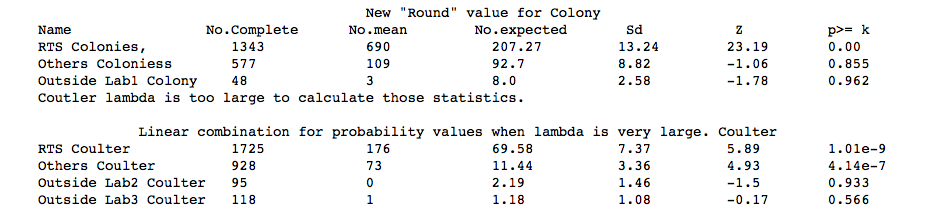
\includegraphics[width=0.9\linewidth]{images/HT_Stat_values.png}
\caption{Approximate Replication of Table 2}
\label{table2}
\end{figure}

    \subsection{Digits Analysis}\label{digits-analysis}

Next, the authors perform some common tests for fraud detection - \textit{terminal
digit analysis} and \textit{pair of equal terminal digits analysis}. These tests
assume that in general insignificant digits of a sample are not very informative.

\subsubsection{Terminal digit analysis}\label{terminal-digit-analysis}

The first test assumes that the last digit in samples of large numbers
($>100$) should empirically show uniform distribution. Also, some previous works
have shown that fabricated data often fail to show such peculiar property.
The authors use the chi-square test for goodness of fit, and get good fits for
the rest data and low $p$-values for the RTS data.
Our results are very similar to theirs, although not identical.

\subsubsection{Equal digits analysis}\label{equal-digits-analysis}

This test assumes that for large numbers empirical frequency of observing a
pair of equal terminal digits is close to $1/10$. Again, the
authors consider only big numbers ($>100$), to ensure the
analysis of insignificant digits. The authors didn't mention the name of tests for this analysis
and but assuming chi-square test for goodness of fit we obtain similar, but not identical results.



\subsubsection{Discussion of
Assumptions}\label{discussion-of-assumptions}

Next, we discuss the assumptions made by the authors:
\begin{itemize}
    \item The authors didn't justify the assumption of Poisson distribution for the underlying data. Beyond our intuition we didn't investigate the validity in detail.
    \item The authors suspected RTS data, but used the suspected data to fit a model and quantify their suspicion. While sometimes this may raise flags, here we agree with the authors that doing so increases the odds in favors the person in question and hence gives us desirable conservative results.
    \item The authors don't discuss why simply filtering the data for counts $>100$ justifies the use of tests for suspicious patterns in insignificant digits. The authors include here additional data, provided by three external sources (two for Coulter counts and one for Colony counts) but all three had relatively small number of data points.
    Despite authors attempts to account for this, we believe that in the current setting, these additional samples do not more compelling evidence. Instead, they added to our confusion. TODO : What confusion?
    \item We reiterate that pooling the data may hide anomalies in the other researchers' data.

\end{itemize}



    \section{Our Analysis}\label{our-analysis}

    As a preliminary test for identifying suspicious datasets, we plot histograms of mid-ratios for the data provided by individual researchers. We also contrast each histogram from the histogram of the pooled data. We only plot the former here. Two important observations can be made:
\begin{figure}[H]
\centering
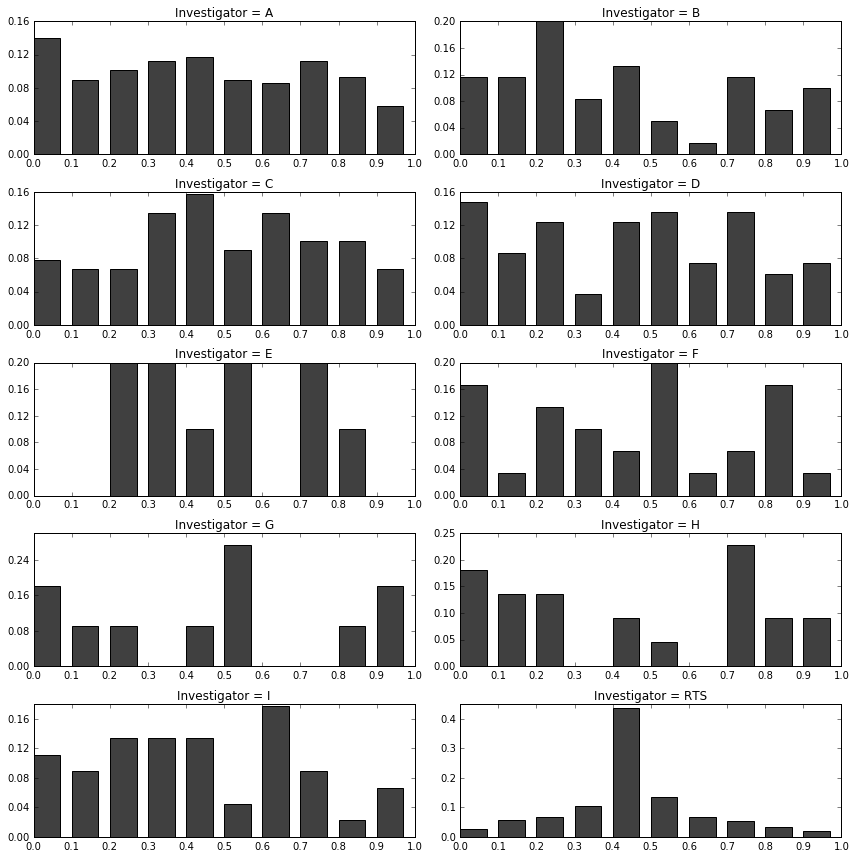
\includegraphics[width=0.8\linewidth]{images/new_mid_ratio.png}
\caption{Individual Histograms for the Colony Data}
\label{ind_mid_ratio}
\end{figure}

\begin{itemize}
\item
  First, the histogram for researchers with labels ``B, C, E, F, G, H, I'' do not
  appear as uniform distribution.
\item
  Second, when the pool includes RTS, the histogram of the pool looks similar to the histogram of RTS due
  to its dominating presence in the pool. Hence, most of the individual researchers look anomalous when 
  contrasted with the pool.
\end{itemize}

These observations point the limitations of assumption of uniform distribution for
mid-ratios and use of visual dissimilarity between histograms of RTS to the pool. Next, we discuss
permutation tests which are free from many such limitations, and come in handy when
little information is available about the distributions of the data.



    \subsection{Permutation Tests}\label{quick-primer-to-permutation-tests}


The problem of determining whether a treatment has an effect is widespread in various real world problems. To evaluate whether a treatment has an effect, it is crucial to compare the outcome when treatment is applied (the outcome for the treatment group) with the outcome when treatment is withheld (the outcome for the control group), in situations that are as alike as possible but for the treatment. This is called the method of comparison. We will describe this method for a specific set up which is relevant for the problem in discussion.

Suppose that we are given two labeled sets of observations - $T$ of them labeled `treatment' and $C$ of them labeled `control'. We assume that the prior of these sets has received a treatment and we wish to test the hypothesis whether this treatment affected the outcomes. In a two-sample permutation test, the data is pooled together
to form a population of size \(N = T+C\).
Next, we decide a test-statistic that can capture the effect of the treatment (if any) between the two groups, and compute it for the given labeled sets. As an example, we can consider the absolute difference between the sample means of the two datasets as the test statistic. Under the null hypothesis that the treatment has no effect, one can analytically derive the distribution of this test statistic. However, often it is easier to empirically approximate rather than numerically compute the distribution. To do so, one repeats the following procedure several times: partition the data into groups of size \(T\) and \(C\) and compute the test statistic contrasting the two datasets. We use the empirical histogram obtained from these repeated experiments, as a proxy for the true distribution of the test statistic. Next, just like typical hypothesis testing, we compute the chances ($p$-value) of observing the test statistic that we computed in the beginning.

When the $p$-value is below a preset significance level, we infer that the treatment has an effect at that level of significance. That is, we conclude that \textit{the
two groups are different to each other} than if we randomly partitioned
the pooled dataset.


    \subsubsection{Results for
Mid-Ratio}\label{permutation-tests-for-mid-ratio}

We set the test statistic to be the difference in
standard deviation of mid-ratios of two datasets. We choose standard deviation because our null and alternative hypothesis for mid-ratio (uniform distribution versus concentration around 0.5) lead to same mean ($0.5$). We expect standard deviation to capture
the \textit{unintentional reduction in spread caused in data due to
intentional adjustments}.

We consider each researcher equivalent to a treatment. We carry these tests in the following fashion. Suppose we want to test if data provided by investigator $A$ were different from the others. Let $n_A$ denote the number of points in $A$'s dataset, and let $N-n_A$ denote the size of the dataset for the rest. These two datasets form the treatment and control group in our permutation tests for contrasting the effect of label `$A$' on the data. We do the procedure explained in the previous section $1000$ times. We obtained a $p$-value of $0.00$ for A, B, D, and RTS; and \(<0.01\) p-value for all others except E,F,G which
indicates that almost all datasets are surprising with respect to this
test-statistic. We would like to note that here a $p$-value of $0.00$ in fact denotes a $p$-value $<0.001$, because of the finite resolution owing to $1000$ tests. We would also like to mention that RTS is still the most surprising if one looks at the location of the test-statistic in the
tails of the distribution.

We also look at \(\ell_1\) distance between the density\footnote{abuse of terminology, used in place of normalized histograms}, and the
\(\ell_1\) distance between the cumulative distribution function (CDF) as the test statistic. Again, we reject several researchers of the lab at a significance level of \(1 \%\). We present all the $p$-values in Figure~\ref{mid_ratio_perm}.

\begin{figure}[H]
\centering
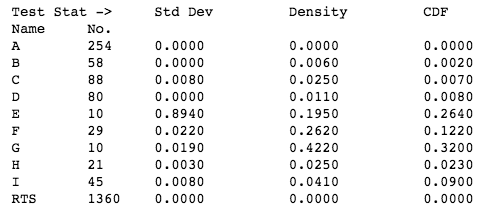
\includegraphics[width=0.8\linewidth]{images/mid_ratio_perm.png}
\caption{Results for Permutation Tests for Mid-Ratio}
\label{mid_ratio_perm}
\end{figure}

{\bf Remark} We would like to mention that when RTS is included in the control group, it constitutes the bulk of the group. As a result, rejecting the null hypothesis is almost equivalent to rejecting the hypothesis that the data of the researcher is same as RTS data. This doesn't help us to make meaningful inferences if we already believed or later found that RTS data was suspicious. To correct for this, we do another set of permutation tests after excluding the RTS data. Now we don't find strong evidence to reject the null hypothesis, and conclude that none of the researchers have any effect at a significance level of $1\%$. However, these set of tests suffer from a bias because of our manual throwing away of 2/3rd data.

\begin{figure}[H]
\centering
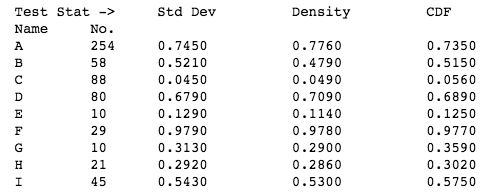
\includegraphics[width=0.8\linewidth]{images/mid_ratio_perm_no_rts.png}
\caption{Results for Permutation Tests without RTS  for Mid Ratios}
\end{figure}

Putting together the pieces, we can conclude that we do have statistical evidence to claim that RTS has suspicious data.

    \subsection{Additional Tests for Digit
Analysis}\label{additional-tests-for-digit-analysis}

For the terminal digit and equal digits tests, we extended the tests done by
the authors to individual members of the lab and performed - chi-square test for goodness of fit for terminal digit; chi-square test for goodness of fit for equal digits and permutation tests for terminal digit. For permutation tests, we used the test statistics listed in the previous section. Results are tabulated in the figures below:

\begin{figure}[H]
\centering
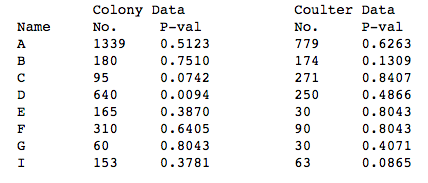
\includegraphics[width=0.7\linewidth]{images/raaz_term_chi_summary.png}
\caption{Chi Square Tests for Terminal Digits in Coulter and Colony
Counts}
\label{cst1}
\end{figure}

\begin{figure}[H]
\centering
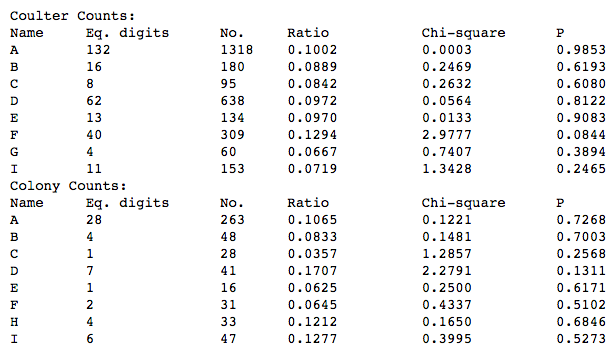
\includegraphics[width=0.9\linewidth]{images/raaz_eq_chi_elaborate.png}
\caption{Chi Square Tests for Equal Terminal Pair in Coulter and Colony
Counts}
\label{cst2}
\end{figure}

Figure~\ref{cst1} shows that $p$-value for $D$, for Coulter Data is less than $1\%$.

\begin{figure}[H]
\centering
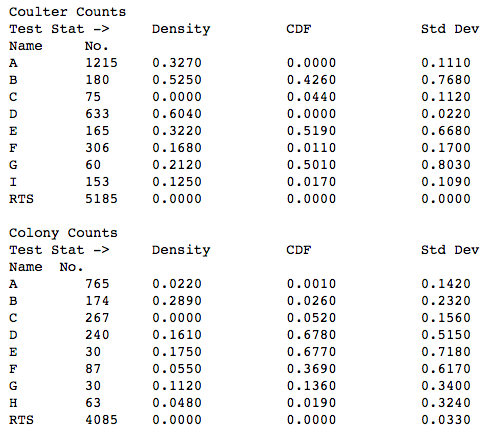
\includegraphics[width=0.7\linewidth]{images/raaz_eq_perm_summary.png}
\caption{Permutation Tests for Terminal Digit Analysis, Coulter counts}
\label{perm2}
\end{figure}

Figure~\ref{perm2} once again confirms that RTS data is suspicious. As before, the huge fraction of data
by RTS contributes towards the low $p$-values for some of the other
researchers. In permutation tests after excluding RTS, none of the researchers look suspicious. We skip the table of the $p$-values for this case.

    \section{Conclusion}\label{conclusion}

    Data fraud is an extremely critical issue in science, engineering and
many other fields. Methods to detect manipulated data are needed to
identify fraudulent research behaviors. Detecting frauds, however, is a
delicate matter. Challenging the credibility of a researcher or of a
scientific work, in fact, can have heavy consequences for all the parties
involved in the process. Methodologies and techniques used in this kind
of work need to be clear and widely accepted. They need to produce
results which leave minimal (ideally no) space to ambiguity. Independently, reproducibility of results is a fundamental element to rule out any doubts that could arise at any time.

In our review, we carefully analyzed the authors' results
and conclusions by: reproducing all the results that have been
discussed in the paper and using additional tests to avoid several assumptions.

TODO : We  out that authors' results are correct, although it has not been
possible to reproduce exactly all the experiments due to lack of some
key pieces of information (for instance how data has been
pre-processed). Moreover, we encourage the use of stronger tools like permutation tests and our demonstration can be considered as a promotion of the same. Such tests help the analysis to get \textit{rid of assumptions}, thereby shifting the focus from debate on assumptions to actual anomalies present and to better understanding of individual
investigator's data (besides the RTS) as to how do they compare to the general data pool.

At the end of our review, we do believe that there is a significant evidence that RTS has suspicious data, but we suggest the authors to collect additional material and investigate more, since some of our tests suggest that other investigator's data have anomalies as well if we do not discount the huge fraction of data given by RTS.

\section*{Acknowledgments} % (fold)
\label{sec:acknowledgments}

We would like to thank the authors H. Pitt and H. Hill for publishing in an open journal, and making the data available for everyone. Also, we would like to thank Prof Philip Stark for his valuable and critical guidelines and timely feedback. We would also like to thank Yuansi Chen for valuable tips with python. As a final note, we would like to claim complete responsibility for all the opinions expressed in this paper.

% section acknowledgments (end)


\bibliographystyle{apalike}
\bibliography{biblio}

    \end{document}
